\documentclass{article}
\usepackage{amsmath}
\usepackage{hyperref}
\usepackage{graphicx}
\usepackage{adjustbox}
\newcommand{\tabincell}[2]{\begin{tabular}{@{}#1@{}}#2\end{tabular}}

\begin{document} %This is where document begins
\begin{titlepage}
\title{EE 232E \\Graphs and Network Flows\\Final Project\\Winter 2016} 
\author{Liqiang Yu, Rongjing Bai, Yunwen Zhu\\
904592975, 204587519, 104593417}  %change your ID here
\date{05-28-2016}
\end{titlepage}

\maketitle
\newpage
\tableofcontents
\newpage

\section{Problem1}\label{prob:p1}
We use python to parse the data in actor\_movies.txt and actress\_movies.txt to merge the information about actor/actress. And when parsing the data, we remove those with less than five movies. Also, we create actor\_id parameter on basis of the order of actor/actress for convenience in mapping for the name. To help mapping with actor\_id and actor's name, we write actor\_id.py and create the correspoinding mapping actor\_id.txt. Finally, there are totally 244300 actor/actress in the merge\_actor.txt and the corresponding parsing program is merge\_actor.py. 


\section{Problem2}
In this problem, we create the weighted directed graph based on the formula $\frac{|Si\cap Sj|}{|Si|}$, where Si = $\lbrace m\mid i\in V$,m is a movie in which i has acted$\rbrace$. We first create a dictionary movie\_actor with the movie as the key and the actors that participate in this movie as the value for quick search. Then we create another dictionary edge\_weight with the two actor\_ids as the key and the number of their same movies as the value. Thus, by traversing each movie with more than two actors involved, we create the edge according to the edge\_weight with the two actor as the vertices and calculated weight. Finally, there are 58026910 edges in this graph in edge\_weight.txt and the corresponding program is create\_graph.py. Also, note that there are many directed edges with weight = 1, that means the movies of that actor totally intersected in the movies of another actor, which fit well in reality as well as the data. 


\section{Problem 3}
We run the pagerank algorithm with damping = 0.85 on our weighted directed graph and we get the names of those in top 10 pageranks with our actor\_id.txt. The names are listed in Table \ref{tb:3_1}.\\

\begin {table}[htbp]
\caption{names of actors with top 10 pageranks}
\begin{adjustbox}{center}
\label{tb:3_1}
\begin{tabular}{|c|c|}
\hline
Flowers, Bess & 0.0001580023\\
\hline
Tatasciore, Fred & 0.0001377731 \\
\hline
Blum, Steve (IX) & 0.0001340366 \\
\hline
Harris, Sam (II) & 0.0001333384 \\
\hline
Jeremy, Ron & 0.0001270027 \\
\hline
Miller, Harold (I) & 0.0001165205 \\
\hline
Lowenthal, Yuri & 0.0001090534 \\
\hline
Downes, Robin Atkin & 0.000104297  \\
\hline
Phelps, Lee (I) & 0.0001012679  \\
\hline
Sayre, Jeffrey & 0.0001006508  \\
\hline
\end{tabular}
\end{adjustbox}
\end{table}

\noindent From the results of Table \ref{tb:3_1}, we just know the name of a few of them, but these top 10  are certainly not the famous stars. Thus, we list the names of famous stars in our opinion and then calculate their corresponding pagerank. Their names and pageranks are listed in Table \ref{tb:3_2}.\\

\begin {table}[htbp]
\caption{names and pageranks of 10 famous stars}
\begin{adjustbox}{center}
\label{tb:3_2}
\begin{tabular}{|c|c|}
\hline
Page, Ellen &  1.172932e-05\\
\hline
Portman, Natalie & 2.365215e-05 \\
\hline
Linney, Laura & 1.848715e-05 \\
\hline
Rudd, Paul (I) & 2.888519e-05 \\
\hline
Dennings, Kat & 9.740525e-06 \\
\hline
Lively, Blake & 3.248758e-05 \\
\hline
Clooney, George & 0.0001090534 \\
\hline
Reynolds, Ryan (I) & 2.143052e-05 \\
\hline
Hanks, Colin & 1.475533e-05 \\
\hline
Radcliffe, Daniel & 1.430697e-05 \\
\hline
\end{tabular}
\end{adjustbox}
\end{table}
\noindent From the Table \ref{tb:3_2}, out of expection, the famous stars we choose are all have a relatively low pagerank, especially when compared with those top 10 pageranks.There are many reasons for this phenomenon that we are not familar with those high pagerank scores. First, due to our subjectivity and our time and country, we may not actually know certain movie stars from other countries but still be well-known in their country. Or these movie stars were really famous in their times but are not sound familar to our generation. Secondly, high rankpage score may not mean great reputation. Those not famous actors tend to try in every kind of movie and act in many movies just as a supporting role. Thus, they do have a closer relationship and connection to many other actors then have a high pagerank score. \\
\\In order to find the 10 most significant pairs, we convert our original directed graph into the undirected one with weight as the mean of the directed edges. Then we sort the weight of all edges, and find out the top 10 as our significant pairs. After that, we use our actor\_id.txt to map into their corresponding names. The names of signicicant pairs are shown in the Table \ref{tb:3_3}.
\begin {table}[htbp]
\caption{10 significant pairs}
\begin{adjustbox}{center}
\label{tb:3_3}
\begin{tabular}{|c|c|}
\hline
Mounir, Dean &  Bailey, Carla Jo\\
\hline
Kim, Su-hyeon (II) & Phillipson, Caspar \\
\hline
Harvey, Nita & Gamal, Mimi \\
\hline
Perlmutter, Kalle & Evans, Kahshanna \\
\hline
Stefancyk, Bryan & de Carvalho, Inalda \\
\hline
Matthews, Liam (III) & DuChesne, Derek \\
\hline
Beltrán, Pedro (I) & McNicol, Valerie (III) \\
\hline
Kasten, Kristina (II) & Gomide, Tânia \\
\hline
Wagner, David (I)& Zhao, Jun (I) \\
\hline
Boulanger, Véronique & Carson, Lisa Nicole \\
\hline
\end{tabular}
\end{adjustbox}
\end{table}
From the Table \ref{tb:3_3}, we can see that these pairs may occur between different actors and  actresses, but these actors all have relatively high weight with their connected edges. That means that they have collaborated with many of other actors in most of their participating movies especially to those whose movies are totally intersected with other actors. However, we actually barely know their names and they do not appear in the top pagerank as well. Actually, their page ranks are relatively low compared with our top pageranks. As, the pageranks do not simplycount for the simple two vertices'links and they consider for the total connectivity.\\
\\
As for the reason why the names in the pairs collaborate in so many movies but we do not know well, there are maybe two of them from our assumption. First, maybe we really are not familiar with them. Actually, when we try to search their names in the Google, we find out that some of them are not our generation. And movies in that age is definitely limited in the numbers, thus actors of that age are more likely to collaborate. Also, some of the actors are from some country that we are not familar with, thus these pairs may sound pretty famous to people from their country. Secondly, these actors may always act in the same kind of movies, thus their chance of co-acting with the same group of people are relatively high.
\section{Problem 4}
We remove all movies with less than 5 actors/actresses in movie-list.txt file, which contains the parsed data with movie actor/actress information.\\
Then we map the actor to each movie and generate movie-edge-list file
The jaccard index is defined as $$J_{ij}=\frac{l_{i} \cap l_{j} }{l_{i}\cup l_{j}}$$
where $l_{i}$ denotes the actor/actress list of movie i.
Then we build the movie network based on the movie-edge-list and add genre, name, rating and director as the attributes of each movie node. There are 244655 nodes in the network.
\section{Problem 5}
After we constructed the network, there are 67 communities in total. The genres of each community occuring higher than 20\% are shown in table \ref{tb:5_1}, not available means there are no genres occuring higher than 20\% in that community.
\begin {table}[htbp]
\caption{The genre of each community}
\label{tb:5_1}
\begin{adjustbox}{center}

\begin{tabular}{|c|c|c}
\hline
1 & drama\\
2 & drama\\
3& short\\
4&drama\\
5&drama\\
6&drama\\
7&adult\\
8&drama\\
9&short\\
10&drama\\
11&drama\\
12&short\\
13&short\\
14&drama\\
15&drama\\
16&drama\\
17&drama\\
18&adult\\
19&drama\\
20&comedy drama\\
21&drama romance\\
22&drama romance\\
23&thriller\\
24&short\\
25&short\\
26&romance\\
27& Not available\\
28&drama\\
29&short\\
30&drama romance\\
31&sci-fi thriller\\
32& short\\
33& short\\
34& drama\\
35& drama\\
\hline
\end{tabular}
\begin{tabular}{|c|c|c}
\hline
36& short\\
37&horror thriller\\
38& thriller\\
39& horror short thriller\\
40& comedy documentary drama\\

41&Not available\\
42&comedy short\\
43&action short\\
44& comedy\\
45&short thriller\\
46&comedy romance\\
47&documentary\\
48&short\\
49&short\\
50&short\\
51&short\\
52&short\\
53&short\\
54&horror short thriller\\
55&short\\
56&drama thriller\\
57& sci-fi short\\
58&adventure thriller\\
59&horror short thriller\\
60&short\\
61& sci-fi short\\
62&adventure crime short\\
63&comedy short thriller\\
64& short\\
63&comedy short thriller\\
64& short\\
65&short\\
66& short\\
67&short\\
\hline

\end{tabular}
\end{adjustbox}
\end{table}
\newpage
\noindent From the statistics, we can see that the most common tags are short and drama.
I think the tags are meaningful because usually one actor/actress tends to act in one or several movies genres. So the tag should represents the genres that the actors/actresses in the lists of the community tends to act in. 
So we can use the genres to tag the community.
However, most of the tag has frequency lower than 0.3 so the tag cannot represents the whole community.
\section{Problem 6}
After searching the community, we found the nearest neighbors.\\

\underline{ Batman v Superman: Dawn of Justice (2016)}:\\
Man of Steel (2013), \\
Into the Storm (2014),\\
Real Steel (2011), \\
Sparkle (2012/I),\\
Salvation Boulevard (2011)\\

\underline {Mission: Impossible - Rogue Nation:}\\
Fan (2015),\\
Phantom (2015)\\
Suffragette (2015), \\Breaking the Bank (2014)\\
The Theory of Everything (2014)\\

\underline{Minions (2015)}\\
The Lorax (2012),\\ Inside Out (2015),\\
Despicable Me 2 (2013), \\Up (2009),\\
Surf’s Up (2007)\\

\noindent Then we check the genres. The three movies belongs to community 3, with short as the genre.
However, they are not short genres, their genres are thriller or sci-fi.
I think this is because there are so many short movies that many of the communities have the tag of short. \\
\\
In fact, as mentioned above, the frequency are less than 0.3 for most of the tag, so it is not weird movie genres are diffrent with the tag of the community.
\section{Problem 7}
To predict the ratings of the above three movies, we use both ratings from their neighbors and from nodes in the same community. The point is how to combine them together. We tried four different methods listed below\\
\\
First of all, let's assign the rates of the neighbor nodes to be $R_n$ and the rates of the nodes in the same community to be $R_c$. The first method is to take the averages of the two rate vectors and then take the average of their averages.
\begin{equation*}
rate = \frac{E(R_n) + E(R_c)}{2}
\end{equation*}
The second method is to take the sum of two rating vectors and then divide them by their sum of the length.
\begin{equation*}
rate = \frac{\sum{R_n}+\sum{R_c}}{\vert{R_n}\vert+\vert{R_c}\vert}
\end{equation*}
The third method considers the edge weight between two nodes when calculate the mean rate of the neighbor nodes, because the edge weight can show how closely each two nodes are connected. Let's assign the edge weight vector to be $E_w$
\begin{equation*}
\begin{aligned}
E'(R_n) = \sum{R_n\cdot E_w}\\
rate = \frac{E'(R_n) + E(R_c)}{2}
\end{aligned}
\end{equation*}
The fourth method is similar to the second method, however we replace the sum to be weighted sum
\begin{equation*}
rate = \frac{\vert{R_n}\vert \cdot \sum{R_n\cdot E_w}+\sum{R_c}}{\vert{R_n}\vert+\vert{R_c}\vert}
\end{equation*}
Table \ref{tb:7} shows the results of the predicting rates with four methods. From the table we can see that the ratings of the three movies tend to be between 5.5 and 6.5.
\begin {table}[htbp]
\caption{Predicting rates with neighborhood and same-community nodes}
\begin{adjustbox}{center}
\label{tb:7}
\begin{tabular}{|c|c|c|c|c|}
\hline
Movie Name&Method 1&Method 2&Method 3&Method 4\\
\hline
Batman v Superman: Dawn of Justice (2016)&6.275912&6.191796&5.383655&6.158682\\
\hline
Mission: Impossible - Rogue Nation (2015)&6.211204&6.189184&5.26059&6.162731\\
\hline
Minions (2015)&6.512196&6.19809&6.360177&6.19361\\
\hline
\end{tabular}
\end{adjustbox}
\end{table}
\section{Problem 8}
In this part, we trained different regression models to predict the movie ratings, the features we use are top 5 actor/actress page ranks computed in Problem 3 and whether the director is in the top 100 directors list. First we fetch the directors of the ``IMDB top 250 movies" and then get the unique 100 directors as well as their rankings. So the feature vector is of length 106. The first 5 items are 5 highest page ranks, the sixth item is a boolean value of whether the director is in the top 100 directors list. If so, the remaining items show his/her ranking. The corresponding item will be 1 according to the ranking.\\
\\
We trained the linear regression model and random forest regression model to predict the ratings and use 10-fold cross validation method to evaluate the results and get rid of the overfitting problem. First we randomly shuffled the whole dataset and splited it into 10 folds. Then each time we use 9 of 10 to do the training and use the remaining 1 part to do the test experiment. We check the root mean square error(RMSE) to evaluate the predicting results.
\subsection{Linear Regression Model}
The root mean square error of the 10-fold cross-validation experiment is shown in figure \ref{fig:8_1}. The average error is 1.27417955416. The predicting rates is shown in table \ref{tb:8_1}

\begin{figure}[htbp]
\centering
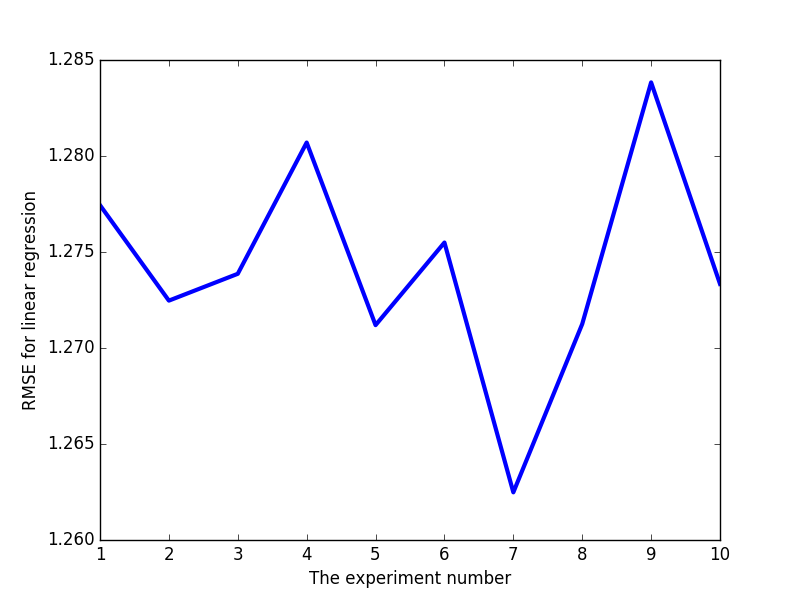
\includegraphics[width=.6\textwidth]{linear.png}
\caption{RMSE for the linear regression model}
\label{fig:8_1}
\end{figure}

\begin {table}[htbp]
\caption{Predicting rates with linear regression model}
\begin{adjustbox}{center}
\label{tb:8_1}
\begin{tabular}{|c|c|}
\hline
Movie Name&Predicting Rate\\
\hline
Batman v Superman: Dawn of Justice (2016)&6.14947715\\
\hline
Mission: Impossible - Rogue Nation (2015)&6.16647388\\
\hline
Minions (2015)&6.16990139\\
\hline
\end{tabular}
\end{adjustbox}
\end{table}

\subsection{Random Forest Regression Model}
The root mean square error of the 10-fold cross-validation experiment is shown in figure \ref{fig:8_2}. The average error is 1.26341071465. The predicting rates is shown in table \ref{tb:8_2}.\\

\begin{figure}[htbp]
\centering
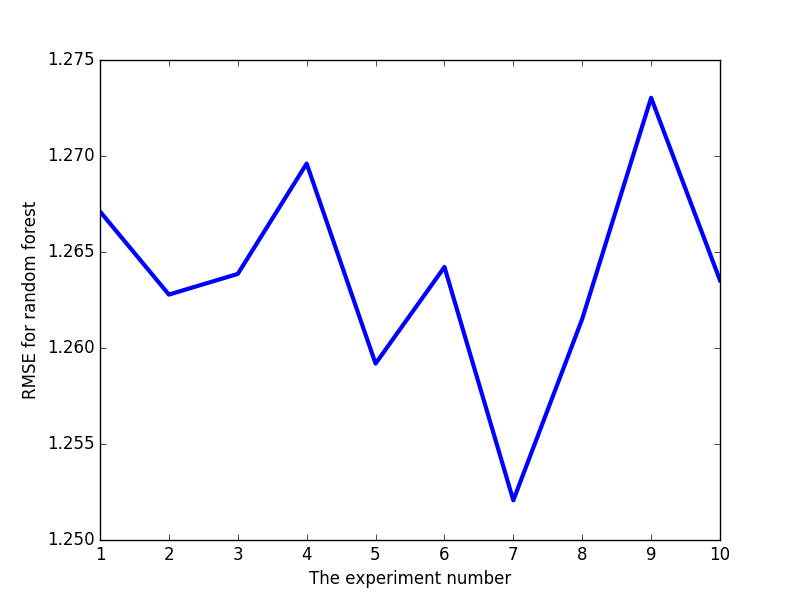
\includegraphics[width=.6\textwidth]{rfr.png}
\caption{RMSE for the random forest regression model}
\label{fig:8_2}
\end{figure}

\begin {table}[htbp]
\caption{Predicting rates with random forest regression model}
\begin{adjustbox}{center}
\label{tb:8_2}
\begin{tabular}{|c|c|}
\hline
Movie Name&Predicting Rate\\
\hline
Batman v Superman: Dawn of Justice (2016)&6.09615458\\
\hline
Mission: Impossible - Rogue Nation (2015)&6.05967233\\
\hline
Minions (2015)&6.13684098\\
\hline
\end{tabular}
\end{adjustbox}
\end{table}

\noindent Basically the two models produced pretty similar results, which are also similar to the results in Problem 7, which means these methods are stable and accurate.
\section{Problem 9}
In this part we constructed a bipartite graph to predict the movie rates. There are 244300 actors and 246335 movies. Each actor/actress is connected to the movies he acted. There are 4023858 edges in the graph. We use four different methods to assign scores to actors based on the movie ratings he acted : mean, max, median and tf-idf. The first three methods are pretty self-explained, we just calculated the mean, max or median of the movie ratings as the actor score.\\
\\
 For tf-idf method, we refered to the tf-idf method in the information retrieval field. When assigning a score to an actor, we give each movie he acted a tf-idf weight as
 \begin{equation*}
 tfidf = \frac{1}{M_i} \times log\frac{A}{A_j}
 \end{equation*}
 where $M_i$ is the number of movies actor i acted, $A$ is the total number of actors and $A_j$ is the number of actors movie $j$ has. Let's assume the normalized tf-idf weight vector for each actor to be $T$, then the score for an actor is
 \begin{equation*}
 score = T^2 \cdot R
 \end{equation*}
 where $R$ is the corresponding movie ratings. Finally we take the average scores of the actors to be the ratings of the movies we want to predict.\\
 \\
 The results of the four methods is shown in table \ref{tb:9}. From the table we can see that mean, median and tf-idf produced similar results, so we believe these three methods are proper for predicting movie rates in the bipartite graph.
 \begin {table}[htbp]
\caption{Predicting rates with bipartite graph}
\begin{adjustbox}{center}
\label{tb:9}
\begin{tabular}{|c|c|c|c|c|}
\hline
Movie Name&Mean&Max&Median&TF-IDF\\
\hline
Batman v Superman: Dawn of Justice (2016)&6.439798&7.864211&6.495263&6.435147\\
\hline
Mission: Impossible - Rogue Nation (2015)&6.541897&8.018889&6.698333&6.537411\\
\hline
Minions (2015)&6.896637&8.686364&7.025&6.907668\\
\hline
\end{tabular}
\end{adjustbox}
\end{table}
\end{document}
